\documentclass[english]{article}
\usepackage[T1]{fontenc}
\usepackage[utf8]{inputenc}
\usepackage{babel}
\usepackage[unicode=true,pdfusetitle,
 bookmarks=true,bookmarksnumbered=false,bookmarksopen=false,
 breaklinks=true,pdfborder={0 0 1},backref=false,colorlinks=false]
 {hyperref}
\usepackage{tabularx}
\usepackage{graphicx}
\graphicspath{{images/}}
\usepackage{svg}
\usepackage{float}
\usepackage{titling}
\renewcommand{\arraystretch}{1.4}
\newcommand{\code}[1]{\texttt{#1}}
\usepackage{array}
\usepackage{caption}

\pretitle{%
	\begin{center}
		\LARGE
		
\includegraphics[width=250pt]{../other/Logo_blu.png}\\[\bigskipamount]~\\[\bigskipamount]
	}
\posttitle{\end{center}}

\begin{document}

\title{Politecnico di Milano\\
 A.A. 2016–2017 \\
Software Engineering 2: “PowerEnJoy” \\
\emph{\textbf{Project Plan}}}

\author{Pietro Ferretti, Nicole Gervasoni, Danilo Labanca}
\date{January 21, 2017}
\maketitle

\newpage

\tableofcontents{}

\newpage

\section{Introduction}

\subsection{Purpose}
The purpose of this document is to provide a detailed analysis of the PowerEnjoy software development project in terms of required cost and time. It highlights the estimation of 
\begin{itemize}
\item project size, calculated using the \emph{Function Points approach} by IBM;
\item project cost and effort, calculated using the \emph{COCOMO II} by Boehm.
\end{itemize}
Given the previous information we elaborate a feasible schedule considering all the necessary activities in detail, thus the best resources' allocation on each one. The last section of the document focuses on handling all the possible risks that could be met during the whole process, from the requirements analysis to the final testing and deployment.


\subsection{Scope}
The aim of this project is to specify and design a new digital management software for PowerEnJoy, a car-sharing service that employs electric cars only.

\paragraph{}
PowerEnJoy will offer a very valuable service to its users, letting them borrow cars to drive around the city freely, as an alternative to their own vehicles and public transport.
Among the advantages of using PowerEnJoy we can note being able to find available cars in any place that is served by our system and having dedicated spots to park in (namely, PowerEnJoy's power grid stations).
Furthermore, thanks to the fact that all the cars that we provide are electrically powered, PowerEnJoy is also very environmentally friendly.

%\paragraph{}
%PowerEnJoy's users, after registering, will be able to reserve, unlock and drive the cars our system will provide. Users will be charged per minute until they park the car in a safe area and end the ride.
%Users will be able to park their car temporarily and use it again later, or end their ride remotely.
%
%Our system will incentivize virtuous behaviour by offering several discounts if certain conditions are met (like charging a car at a power grid station).

\newpage
\subsection{List of Definitions and Abbreviations}

\subsubsection{Definitions}

%\begin{itemize}
%%\item{\textit{Guest}: a person that is not registered to the system.}
%\item{\textit{User}: a person that is registered to the system. Users can log in to the system with their email or username and their password. Their first name, last name, date of birth, driving license ID are stored in the database.}
%\item{\textit{Safe area}: a location where the user can park and leave the car. Users can end their ride and park temporarily only in these locations. The set of safe areas is predefined by the system.}
%\item{\textit{Power grid station} or \textit{Charging station}: a place where cars can be parked and plugged in. While a car is plugged in a power grid station its battery will be recharged. Power grid stations are by definition safe areas.}
%\item{\textit{Available car}: a car that is currently not being used by any user, and has not been reserved either. Available cars are in good conditions (not dirty nor damaged) and don't have dead batteries.}
%\item{\textit{Reservation}:
%	\begin{itemize}
%		\item{the operation of making a car reserved for a user, i.e. giving permission to unlock and use the car only for that user, forbidding reservations by other users.}
%		\item{the time period between the moment a reservation is requested and the moment the user unlocks the car, or the reservation is canceled.}
%	\end{itemize}
%}
%\item{\textit{Ride}: the time period from the moment a reserved car is unlocked to the moment the user notifies that he wants to stop using the car and closes all the doors. A ride doesn't stop when a car is temporarily parked, but continues until the user chooses to leave the car definitely.}
%%\item{\textit{Possession}: users that have reserved and unlocked a car are said to have possession of the car. While a user has possession of a car they are the only person that can drive it, lock or unlock it, and no other person can take possession of it until the user frees it. Users lose possession of a car when their ride ends.}
%\item{\textit{Temporary parking}: the act of parking a car in a safe area and, after notifying the system, locking it and leaving it for a finite amount of time. The user that does this retains the right to use the car and can unlock it later to use it again.}
%\item{\textit{Bill}: a record of the money owed by the user at the end of a ride.}
%%\item{\textit{Outstanding bill}: a bill that hasn't been paid yet. }
%\item{\textit{Suspended user}: a user that cannot reserve or use cars. Usually users are suspended because they have outstanding bills that have not been paid.}
%\item{\textit{Payment method}: a way to transfer money from the user to the system. Our system will only accept credit cards and online accounts like Paypal.}
%\item{\textit{Payment API}: an interface to carry out money transactions, offered by the external provider associated to the payment method used (e.g. a bank).}
%\item{\textit{CAN bus}: a vehicle bus standard designed to allow micro controllers and devices to communicate with each other.}
%\end{itemize}

\subsubsection{Acronyms}
\begin{itemize}
\item \textbf{ITPD}: Integration Test Plan Document
\item{\textbf{DD}: Design Document}
\item{\textbf{RASD}: Requirements Analysis and Specification Document}
\item{\textbf{DB}: Database}
%\item{\textbf{CVV}: Card Verification Value}
%\item{\textbf{DOB}: Date of birth}
\item{\textbf{PGS}: Power Grid Station}
\item{\textbf{GPS}: Global Positioning System}
\item{\textbf{API}: Application Programming Interface}
\item{\textbf{ISDTN}: International Standard Date and Time Notation}
\item \textbf{EM}: Effort Multiplier
% anche tutti i cost driver, ecc.?
%\item{\textbf{CAN bus}: Controller Area Network bus}
\item {\textbf{FP}: Function Points}
\item \textbf{ILF}: Internal Logic File
\item \textbf{ELF}: External Logic File
\item \textbf{EI}: External Input
\item \textbf{EO}: External Output
\item \textbf{EQ}: External Inquiries
%\item \textit{DBMS}: Database Management System
%\item \textbf{ETA}: Estimated Time of Arrival
\item \textbf{UI}: User Interface
\end{itemize}

\subsubsection{Abbreviations}
\begin{itemize}
	\item{\textbf{Tx}: Task}
\end{itemize}

\subsection{List of Reference Documents}

\begin{itemize}
	\item{Requirements analysis and specification document: “RASD.pdf”}
	\item{Design document: “DD.pdf”}
	\item{Integration testing document: “ITPD.pdf”}
	\item{Project description document: “Assignments AA 2016-2017.pdf”}
	\item{Example document: “Project planning example document.pdf”}
	\item{“COCOMO II -- Model Definition Manual”, version 2.1, 1995-2000, Center for Software Engineering, USC} % http://csse.usc.edu/csse/research/COCOMOII/cocomo2000.0/CII_modelman2000.0.pdf
\end{itemize}

\section{Project size, cost and effort estimation}

%TODO descrizione sezione

\subsection{Size estimation: function points}
Function points are useful in expressing the number of business functionalities our software has to provide to a user, and are used to compute an estimation of its size.
They can be identified and categorized into one of five types: outputs, inquiries, inputs, internal files, and external interfaces. Each functional requirement is then assessed for complexity and assigned a number of function points.\\
We based our computation on tables and values in the \emph{COCOMO II Model Definition Manual v. 2.1}.

\subsubsection{Internal Logic Files (ILFs)}

Internal Logic Files are all the kinds of data used and managed by the application in  order to offer the expected functions.\\
Data will be organized in the following tables in the DB:

\begin{itemize}

	\item \textbf{User} : name, surname, username, password, dob, email, licenseID, cvv, cardNumber, accountStatus

	\item \textbf{Bill} : associatedLicense, total, date, rideID, carID, paymentStatus

	\item \textbf{Car} : model, plate, ID, available, issues

	\item \textbf{Report} :carID, description, associatedLicense, date

	\item \textbf{Safe area} : latitude, longitude, ID

	\item \textbf{PGS} : latitude, longitude, ID

	\item \textbf{Plug} : availability, ID

	\item \textbf{Reservation} : ID, associatedLicense, carID, date, status

	\item \textbf{Ride} : ID, associatedLicense, associatedBill, date, status, ridingTime, carID

\end{itemize}

The software will operate directly on the single rows and tables, joining them appropriately if needed.\\
All this data is modeled in simple structures so its complexity can be considered low (referring to tables).

\begin{center}
	\begin{tabular}{ |p{8cm}|m{2cm}|p{1cm}| }
		\hline
		\multicolumn{1}{|c|}{\textbf{ILF}} & \multicolumn{1}{c|}{\textbf{Complexity}} & \multicolumn{1}{c|}{\textbf{FPs}} \\
		\hline
		User & Low & 7 \\
		\hline
		Bill & Low & 7\\
		\hline
		Car & Low & 7\\
		\hline
		Report & Low & 7\\
		\hline
		Safe area & Low & 7\\
		\hline
		PGS & Low & 7\\
		\hline
		Plug & Low & 7\\
		\hline
		Reservation & Low & 7\\
		\hline
		Ride & Low & 7\\
		\hline
		\multicolumn{2}{|l|}{\textit{Total}} & \multicolumn{1}{l|}{63} \\
		\hline
	\end{tabular}
\end{center}

\paragraph{}

\subsubsection{External Logic Files (ELFs)}

The situations where our system demands external data are when it needs information regarding geolocation, or when it must guarantee the legal validity of driving licenses.\\
In particular:

\begin{itemize}
	\item \textbf{GraphHopper API}:
		\begin{itemize}
			\item{Given the string containing the address, the API returns a pair of float numbers representing the coordinates of that location.}
			\item{Given two pair of coordinates, the API return a float representing the time necessary to travel between two positions.}
		\end{itemize}
	\item \textbf{Eucaris API}:
		\begin{itemize}
			\item{Given name, surname, driving license ID and expiration date as string,s the API returns a boolean value representing the correspondence with an existing driving license in Eucaris DB.}
		\end{itemize}
\end{itemize}

In the final analysis, as the data involved are only strings and numbers of small size, we can assess these logic files as low complexity.\\

\begin{center}
	\begin{tabular}{ |p{8cm}|m{2cm}|p{1cm}| }
		\hline
		\multicolumn{1}{|c|}{\textbf{ELF}} & \multicolumn{1}{c|}{\textbf{Complexity}} & \multicolumn{1}{c|}{\textbf{FPs}} \\
		\hline
		Reverse geocoding & Low & 5 \\
		\hline
		Isochrone distance & Low & 5\\
		\hline
		Driving Licenes legal validity & Low & 5\\
		\hline
		\multicolumn{2}{|l|}{\textit{Total}} & \multicolumn{1}{l|}{15} \\
		\hline
	\end{tabular}
\end{center}

\paragraph{}
\subsubsection{External Inputs (EIs)}

PowerEnjoy offers a diverse set of functionalities that requires the user's input.\\
In particular:

\begin{itemize}

	\item{\textbf{Login}: this functionality demands only two strings as parameters, the username and the password, that will be compared with the ones stored in the DB. We can consider this a low complexity operation.}
	
	\item{\textbf{User update}: this functionality includes a collection of operations that allow to modify each aspect of the user's profile. The input data are simple strings. Since the possibilities are conspicuous and the different elaborations aren't basic, and futhermore they interest several components, we can regard this functionality as an average complexity operation.}
	
	\item{\textbf{Pay bill} (automatically/manually): this is one of the most complex operations. It involves internal components and external APIs and it demands two numbers as input. Given the relevance of the operation and the parts interested, we can consider this as a high complexity operation.}

	\item{\textbf{Create reservation}: this functionality requires as input the user ID and car ID that we can consider simple, but its complexity is due to the components involved. At the moment of the creation, the application verifies if the user is suspended, and after that the availability field of the tuple representing the car is modified and the car itself is put in order to be unlocked. Moreover the reservation made by the user is inserted in the list of reservations. We classify the operation as having average complexity.}

	\item{\textbf{Cancel reservation}: the analysis made for the previous functionality is also valid for this one. The operations are comparable as elaboration, and thanks to this the complexity of this functionality is average.}

	\item{\textbf{Start ride}: this action is very simple as it needs only the user ID and the car ID and starts the tally for the duration of the ride. Made this consideration we can see this functionality as low complexity.}

	\item{\textbf{End ride}: this functionality is one of the most complex ones because it involves many different components, and starts the payment process (that has high complexity on its own). When a ride ends the car is set as available in the DB, it creates a bill for the user and initiates the payment. As usual the inputs are simple strings.}

	\item{\textbf{Park}: this functionality expects as inputs the position of the car that are a pair of numbers, the user ID and the car ID. In the elaboration of this data the components interested are the internal car system and the DB to verify if the position belongs to a safe area. Due to the urgency of the action this functionality can be classified as average complexity.}

	\item{\textbf{Unlock car}: this functionality receives the position of the user and his ID, and the car ID. After that the system proceeds to notify the car to open the doors and calls the \textit{start ride} function. Since it includes another functionality and communicates with the car we classify this functionality as average complexity.}

	\item{\textbf{Update car}: this functionality requires only two parameters: the car ID and the status to be updated. This operation mainly involves the DB. For these reasons this functionality has low complexity.}

	\item{\textbf{Update plug}: as the previous functionality, this one too only requires two parameters and affects the DB. So it's a low complexity functionality.}

	\item{\textbf{Set car available}: as the previous functionality, this one too only requires two parameters and affects the DB. So it's a low complexity functionality.}

	\item{\textbf{Set car available}: as the previous functionality, this one too only requires two parameters and affects the DB. So it's a low complexity functionality.}

	\item{\textbf{Report issue}: this functionality receives the parameters of a form as input, so a set of strings, and modifies the status of the car in the DB and the car record itself. We can consider this functionality as an operation with average complexity.}
\end{itemize}

	\begin{center}
	\begin{tabular}{ |p{8cm}|m{2cm}|p{1cm}| }
		\hline
		\multicolumn{1}{|c|}{\textbf{EI}} & \multicolumn{1}{c|}{\textbf{Complexity}} & \multicolumn{1}{c|}{\textbf{FPs}} \\
		\hline
		Login & Low & 3 \\
		\hline
		User update & Average & 4\\
		\hline
		Pay bill & High & 6x2\\
		\hline
		Create reservation & Average & 4\\
		\hline
		Cancel reservation & Average & 4\\
		\hline
		Start ride & Low & 3\\
		\hline
		End ride & High & 6\\
		\hline
		Park & Average & 4\\
		\hline
		Unlock car & Average & 4\\
		\hline
		Update car & Low & 3\\
		\hline
		Update plugs & Low & 3\\
		\hline
		Set car unavailable & Low & 3\\
		\hline
		Set car available & Low & 3\\
		\hline
		Report issue & Average & 4\\
		\hline
		\multicolumn{2}{|l|}{\textit{Total}} & \multicolumn{1}{l|}{60}\\
		\hline
	\end{tabular}
\end{center}

\subsubsection{External Inquiries (EQs)}

In this section we will discuss about External Inquiries that could be defined as elementary processes that send data or control information outside the application boundary. An external inquiry is a functionality that provides information to a user after a query or a request, by retrieving data from an ILF or ELF. \\
In our case we have: 

\begin{itemize}
	\item{\textbf{Get user info}: it returns a set of strings representing the user's info, from the DB.}

	\item{\textbf{Get bills}: it returns a list of bills (mainly strings) owned by the user, retrieved from the DB.}

	\item{\textbf{Car/PGS/Safe area search with position}: in this case the function needs a parameter that is a pair of numbers and returns a list extracted from the DB. For these operations there are some computations to do. Because of that we classify these actions having average complexity.}

	\item{\textbf{Car/PGS/Safe area search with address}: as for the previous cases, these functionalities also have an average complexity, also considering that there are interactions with the \textit{GraphHopper API} in order to convert the address in coordinates.}

	\item{\textbf{Money Saving Option}: this is one of the most complex operations, because it has extract information from the DB and do complex elaborations to find the best solution.}

	\item{\textbf{Cars in need of maintenance}: this is a simple functionality that is employed by maintenance operators and returns a list of cars that are unavailable.}
\end{itemize}


\begin{center}
	\begin{tabular}{ |p{8cm}|m{2cm}|p{1cm}| }
		\hline
		\multicolumn{1}{|c|}{\textbf{EQ}} & \multicolumn{1}{c|}{\textbf{Complexity}} & \multicolumn{1}{c|}{\textbf{FPs}} \\
		\hline
		Get user info & Low & 3 \\
		\hline
		Get bills & Low & 3\\
		\hline
		Car/PGS/Safe area search with position & Average & 4x3\\
		\hline
		Car/PGS/Safe area search with address & Average & 4x3\\
		\hline
		Money Saving Option & High & 6\\
		\hline
		Cars in need of maintenance & Low & 3 \\
		\hline
		\multicolumn{2}{|l|}{\textit{Total}} & \multicolumn{1}{l|}{39}\\
		\hline
	\end{tabular}
\end{center}

\paragraph{}

\subsubsection{External Outputs (EOs)}

The situation our system needs to notify external agents are the following:

\begin{itemize}
	\item{\textbf{Un/Lock car}}

	\item{\textbf{Car update}}
\end{itemize}

The first case has a low complexity, while the second is a little bit more complex because it needs to extract the information from the car.

\begin{center}
	\begin{tabular}{ |p{8cm}|m{2cm}|p{1cm}| }
		\hline
		\multicolumn{1}{|c|}{\textbf{EO}} & \multicolumn{1}{c|}{\textbf{Complexity}} & \multicolumn{1}{c|}{\textbf{FPs}} \\
		\hline
		Un/Lock car & Low & 4x2 \\
		\hline
		Car update & Average & 5\\
		\hline
		\multicolumn{2}{|l|}{\textit{Total}} & \multicolumn{1}{l|}{13}\\
		\hline
	\end{tabular}
\end{center}

\newpage
\subsubsection{Overall estimation}

\paragraph{}
\begin{center}
	\begin{tabular}{|p{5cm}|p{1cm}|}
		\hline
		\textbf{Function Type} & \textbf{FPs} \\
		\hline
		Internal Logic Files & 63 \\
		External Logic Files & 15 \\
		External Inputs & 60 \\
		External Inquiries & 39 \\
		External Outputs & 13 \\
		\hline
		\textit{Total} & 190 \\
		\hline
	\end{tabular}
\end{center}

This table contains a recap of the evaluations of each type of function point.\\
By enumerating the function points we can find an estimation for the number of lines of code the software will have.
The formula we are going to use is:


\begin{center}
$SLOC = AVC \times FPs$
\end{center}
where

$ AVC $ is a language dependent factor

$ FPs$ is equal to the number of function points ($190$ in our case)

\paragraph{}
Since our system will be developed using the Java Enterprise Edition stack, we will take 46 as the AVC factor (following standard empirical measurements\footnote{\href{http://www.qsm.com/resources/function-point-languages-table}{http://www.qsm.com/resources/function-point-languages-table}} for an average project). 

In the end, we have:

\begin{center}
$SLOC = 8740$ lines of code
\end{center}


\newpage
\subsection{Cost and effort estimation: COCOMO II}

To estimate the cost and effort required to develop the software we use the COCOMO II model\footnote{\href{http://csse.usc.edu/csse/research/COCOMOII/cocomo2000.0/CII\_modelman2000.0.pdf}{http://csse.usc.edu/csse/research/COCOMOII/cocomo2000.0/CII\_modelman2000.0.pdf}}.

Since the architecture and structure of our software has been already designed and thought out in details in the Design Document, we will use the COCOMO II Post-Architecture Model.


\subsubsection{Scale Factors}

Five scale factors are used to compute the scale exponent $E$, that accounts for the economies or diseconomies of scale that characterize our project.

If $E$ < 1.0, the project exhibits economies of scale, otherwise diseconomies of scale are present (usually because of communications overhead or large-system integration overheads).

\paragraph{}
There are five scale factors: \textit{Precedentedness}, \textit{Development Flexibility}, \textit{Architecture/Risk Resolution}, \textit{Team Cohesion}, \textit{Process Maturity}. Each of them can be classified on a scale from "Very Low" to "Very High".

%TODO tabella dove ci sono tutti i valori?

% rate, judge, classify, assess, consider

\paragraph{Scale factors:}
\begin{itemize}
	\item \textbf{Precedentedness (PRED):} 
	Precedentedness is high if the product is similar to previously developed projects.
	
	We never developed anything similar and on the same scale, so we rate this factor as \textit{Very Low}.
	
	\item \textbf{Development Flexibility (FLEX):} 	
	This factor measures how rigidly must the software conform with the requirements and the interface specifications.
	
	We do follow the requirements to reach all of the customer's goals, but this is not a project were extreme rigorousness is necessary due to hardware constraints or danger to things or people. We rate this as \textit{Nominal}.
	
	\item \textbf{Architecture / Risk Resolution (RESL):} High if the architecture has been carefully designed, the risks have all been identified and accounted for, and there is low uncertainty and risk in general.
	
	We consider the architecture we developed as robust and detailed, and the risk management plan covers most of the problem we could encounter during the development, with detailed strategies for all relevant risks. We rate this factor as \textit{High}.
	
	\item \textbf{Team Cohesion (TEAM):} 
	This factor quantifies the personnel's experience as a team, willingness to work together and the presence of a shared vision and commitment to the project.
	
	We, as the developers for this project, have already worked together multiple times and have a lot of experience working as a team; we therefore rate this factor as \textit{Very High}.
	
	\item \textbf{Process Maturity (PMAT):} this factor follows the Capability Maturity Model (CMM), associating a rating to each CMM level. 
	
	We are not at a process level where everything is quantified and optimized yet, but we do follow clear, defined methods. It is reasonable to judge it as a level 3 in the CMM ("defined"), equivalent to a \textit{High} rating.
\end{itemize}

\begin{center}
	\begin{tabular}{|p{6cm}|p{2cm}|p{1cm}|}
		\hline
		\multicolumn{1}{|c|}{\textbf{Scale Factor}} & \multicolumn{1}{c|}{\textbf{Level}} & \multicolumn{1}{c|}{\textbf{Value}} \\
		\hline
		Precedentedness (PREC) & Very Low & 6.20 \\
		Development Flexibility (FLEX) & Nominal & 3.04 \\
		Architecture / Risk Resolution (RESL) & High & 2.83 \\
		Team Cohesion (TEAM) & Very High & 1.10 \\
		Process Maturity (PMAT) & High & 3.12 \\
		\hline
		\multicolumn{2}{|l|}{\textit{Total}} & 16.29 \\
		\hline
	\end{tabular}
	\captionof{table}{COCOMO II values for the scale factors.}
\end{center}


\subsubsection{Cost Drivers}

To accurately determine the amount of effort the development will require, the nominal, baseline effort is adjusted with several Effort Multipliers. In the Post-Architecture Model these are also known as \textit{cost drivers}. 

\paragraph{}
There are 17 different cost drivers, and each one can have a rating ranging from "Very Low" to "Very High". The ratings map directly to a multiplicative factor, that can increase or decrease the estimated amount of effort needed to develop the software.

%TODO dividere i cost drivers per categorie di fattori?

\paragraph{Product Factors:}

\begin{itemize}

\item \textbf{Required Software Reliability (RELY):} 

This factor conveys the necessity for our software to work correctly over a long period of time. If the effect of a software failure is only slight inconvenience then RELY is very low. If a failure would risk human life then RELY is very high.

Our software doesn't control the cars' hardware (with the exception of the locking/unlocking mechanism), so there's no worry that failures could cause accidents or injuries to our customer, and the unlikely cases of people getting stuck in cars can be avoided with simple failsafes (being able to unlock the car from the inside). In case of a system failure the only negative effect would be that our service would be unavailable for our customers, but we judge this to lead to at most moderate losses. We consider this driver \textit{Nominal}.

\item \textbf{Database Size (DATA):} This cost driver attempts to capture the effect large test data requirements have on product development. The rating is determined by calculating D/P, the ratio of bytes in the testing database to SLOC in the program.

We believe our testing database will be at least 100MB of size. Given that we estimated the source code to be around ~9000 lines long, this brings the D/P ratio to a order of magnitude of $10^4$.

Following the indications of the COCOMO II model, this is equivalent to a rating of \textit{Very High}.

%DATA ->  
%dimensioni database: ordine di grandezza database di test 1GB % (meno?)
%linee di codice: ~9000
%D/P = ~10\^9/10\^4 = 1*10\^5 = 100'000
%Very High -> 1.28

\item \textbf{Product Complexity (CPLX):} To evaluate complexity we need to weigh five areas: control operations, computational operations, device-dependent operations, data management operations, and user interface management operations.

Our software doesn't need complex computations or special operations, except for some data handling.
Checking on the COCOMO tables for product complexity and averaging the results we judge the complexity rating to be \textit{Nominal}.

%CPLEX ->
%- control operations:
%Very High
%- computational operations
%Nominal
%- device-dependent operations
%Low
%- data management operations
%High
%- User Interface management operations
%nominal
%
%(5+3+2+4+3)/5=3.qualcosa
%totale Nominal 1.00

\item \textbf{Developed for Reusability (RUSE):} This cost driver accounts for the additional effort needed to construct components
intended for reuse on current or future projects.

We have no requirements asking us to develop code ready to be reused in other projects or products. No reusability constraints.
We have no requirements for developing code to be used in other products, and know of no plans for new or future projects. Therefore we have very little reusability constraints and we can rate this driver as \textit{Low}.

%RUSE -> none, not in requirements, Low 0.95

\item \textbf{Documentation Match to Life-Cycle Needs (DOCU):} The rating scale for the DOCU cost driver is evaluated in terms of the suitability of the project’s documentation to its life-cycle needs.

We have no specific instructions about the software's documentation, so we plan to include the right amount of documentation without wasting too much effort to produce more than what will be actually needed for the extent of the product life-cycle. This factor is rated as \textit{Nominal}.

%DOCU -> right-sized to life cycle needs, Nominal 1.00

\end{itemize}

\paragraph{Platform Factors:}

\begin{itemize}
\item \textbf{Execution Time Constraint (TIME):} This is a measure of the execution time constraint imposed upon a software system. The rating is expressed in terms of the percentage of available execution time expected to be used by the system or subsystem consuming the execution time resource.

We want our software to be as responsive and efficient as possible, without requiring extremely performant hardware. We expect to occupy 3/4 of all the available processing power on an any given moment. Following the COCOMO II guidelines, this is equivalent to a \textit{High} rating.

%TIME -> un numero a caso High 1.11

\item \textbf{Main Storage Constraint (STOR):} This rating represents the degree of main storage constraint imposed on a software system or subsystem.

In today's terms storage is easily, readily available and very cheap. We will have no problem acquiring enough hardware for all of our storage needs, so this factor can be safely seen as \textit{Nominal}.

%STOR -> abbiamo un sacco di spazio, Nominal 1.00

\item \textbf{Platform Volatility (PVOL):} “Platform” is used here to mean the  hardware and software (OS, DBMS, etc.) which our software will have to rely on to work. This rating ranges from low, if there is a major change every 12 months, to very high, in the case of a major change every two weeks.

We want our software to be kept updated to fix bugs and possible vulnerabilities. A major update every 2 months and minor ones every week seems reasonable. This corresponds to a rating of \textit{High}.

%PVOL -> major update 2 mesi, High 1.15

\end{itemize}

\paragraph{Personnel Factors:}

\begin{itemize}
\item \textbf{Analyst Capability (ACAP):} Analysts are the people who work on requirements, high-level design and detailed design. The major attributes that should be considered in this rating are analysis and design ability, efficiency and thoroughness, and the ability to communicate and cooperate.

Even if we believe our analysis to be sound, we consider ourselves to be no more than average analysts. This driver is \textit{Nominal}.
%ACAP -> Nominal 1.00

\item \textbf{Programmer Capability (PCAP):} This driver accounts for the developers ability, efficiency and thoroughness, and the ability to communicate and cooperate.

We are very confident in our abilities in programming, and we know that we can work really well as a team. We see nothing wrong in choosing a \textit{Very High} for this driver.

%PCAP -> capacissimi con java e che talento Very High 0.76

\item \textbf{Personnel Continuity (PCON):} The rating scale for PCON is in terms of the project’s annual personnel turnover: from
3\%, a very high continuity, to 48\% in particular settings of high turnover.

We are going to be the ones developing this piece of software, and we are pretty dedicated to following this through until the end. We rate the probability of any of us leaving as negligible; therefore we predict the continuity of the project development to be \textit{Very High}.

%PCON -> no turnover, Very High 0.81

\item \textbf{Applications Experience (APEX):} The rating for this cost driver is dependent on the level of applications experience possessed by the project team developing the software system or subsystem. The ratings are defined in terms of the project team’s equivalent level of experience with this type of application.

We sincerely don't have much experience with this type of application, except for basic client-server architectures. This driver can be rated as \textit{Low}.

%APEX -> poca esperienza, Low 1.10

\item \textbf{Platform Experience (PLEX):} This factor expresses the experience with using powerful platforms, including graphic user interface, database, networking, and distributed middleware frameworks.

We have very little experience with database, networking, and distributed middleware software. We have to rate this as \textit{Very Low}.

%PLEX -> veeery low, Very Low 1.19

\item \textbf{Language and Tool Experience (LTEX):} This is a measure of the level of programming language and software tool experience of the project team developing the software system or subsystem.

We have a good amount of experience with Java, but not as much with the J2EE framework. We can consider this as \textit{Nominal}, not too high and not too low.

%LTEX -> Nominal, 1.00

\end{itemize}

\paragraph{Project Factors:}

\begin{itemize}

\item \textbf{Use of Software Tools (TOOL):} This driver measures the capabilities of the tools and editors the developers are going to use.

Modern Java IDEs like Eclipse and Netbeans are very advanced and perfectly fit into the COCOMO classification for "strong, mature, proactive life-cycle tools, well integrated with processes, methods, reuse". What these IDEs lack can be easily integrated with additional software and plugins, like Sonar. We believe a rating of \textit{Very High} to be appropriate.

%TOOL -> abbiamo eclipse, Very High 0.78

\item \textbf{Multisite Development (SITE):} This driver is a value averaging of two factors: site collocation (from fully collocated to international distribution) and communication support (from surface mail and some phone access to full interactive multimedia).

As developers we are approximately located in the same metro area, and are able to meet whenever it is needed to work together. Furthermore we have access to many different communication tools, like emails, messaging applications, source control software and web-based project management applications. We rate this factor as \textit{High}.

%SITE -> same city or metro area, High 0.93

\item \textbf{Required Development Schedule (SCED):} This rating measures the schedule constraint imposed on the project team developing the software. The ratings are defined in terms of the percentage of schedule stretch-out or acceleration with respect to a nominal schedule for a project requiring a given amount of effort.

We have no specific requirements or constraints on development time and schedules.
We can keep the typical time needed for development, with no schedule acceleration or stretching. This factor is therefore \textit{Nominal}.

%SCED -> boh, teniamo una schedule non accelerata, Nominal 1.00

\end{itemize}

\begin{center}
	\begin{tabular}{|p{8cm}|p{2cm}|p{1cm}|}
		\hline
		\multicolumn{1}{|c|}{\textbf{Cost Driver}} & \multicolumn{1}{c|}{\textbf{Level}} & \multicolumn{1}{c|}{\textbf{Value}} \\
		\hline
		Required Software Reliability (RELY) & Nominal & 1.00 \\
		Database Size (DATA) & Very High & 1.28 \\
		Product Complexity (CPLX) & Nominal & 1.00 \\
		Required Reusability (RUSE) & Low & 0.95 \\
		Documentation match to lyfe-cycle needs (DOCU) & Nominal & 1.00 \\
		Execution Time Constraint (TIME) & High & 1.11 \\
		Main Storage Constraint (STOR) & Nominal & 1.00 \\
		Platform Volatility (PVOL) & High & 1.15 \\
		Analyst Capability (ACAP) & Nominal & 1.00 \\
		Programmer Capability (PCAP) & Very High & 0.76 \\
		Personnel Continuity (PCON) & Very Low & 0.81 \\
		Application Experience(APEX) & Low & 1.10 \\
		Platform Experience (PLEX) & Very Low & 1.19 \\
		Language and Tool Experience (LTEX) & Nominal & 1.00 \\
		Usage of Software Tools (TOOL) & Very High & 0.78 \\
		Multisite Development (SITE) & High & 0.93 \\
		Required Development Schedule (SCED) & Nominal & 1.00 \\
		\hline
		\multicolumn{2}{|l|}{\textit{Total}} & 0.907 \\
		\hline
	\end{tabular}
	\captionof{table}{COCOMO II values for the cost drivers.}
\end{center}

\newpage
\subsubsection{Effort equation}

We use the formula from the COCOMO II Post-Architecture Model to estimate the effort needed for the development.
\\We will refer to the estimated Person-Month effort needed to develop the code as $PM$.


\begin{center}
$ PM = A \times Size^E \times \prod_{i=1}^{17} EM_i $
\end{center}

\begin{center}
$ E = B + 0.01 \times \sum_{j=1}^{5} SF_j $
\end{center}
where

$ A = 2.94 $ is a calibrated constant 

$ B = 0.91 $ is a calibrated constant

$EM_i$ are the effort multipliers (cost drivers)

$SF_j$ are the scale factors

$Size$ is the estimated thousands of lines of source code (\textit{KSLOC})


\paragraph{}
By substituting the numbers obtained in the previous analysis and the COCOMO II model we have

\begin{center}
$E = 0.91 + 0.01 \times 16.29 = 1.07$
% E>1 --> diseconomy of scale, troppo overhead di comunicazione ecc.
\end{center}

\begin{center}
$PM = 2.94 \times 8.7^{1.06} \times 0.907 = 26.41$ person-months
\end{center}

We can see that $E > 1$, displaying diseconomies of scale. This is mainly because this project is mostly unprecedented.

\subsubsection{Schedule estimation}

According to the COCOMO II model, we can estimate the approximate is the time necessary to develop the code in calendar months. We will refer to the estimate as $TDEV$.\\
Assuming no schedule compression or stretching-out,

\begin{center}
	$TDEV = C \times PM^F$
\end{center}

\begin{center}
	$F = D + 0.2 \times (E-B)$
\end{center}
where

$B = 0.91$ is a calibrated constant

$C = 3.67$ is a calibrated constant

$D = 0.28$ is a calibrated constant

$E$ is the scaling exponent for the effort equation

$PM$ is the number of person-months obtained in the effort estimation
\paragraph{}
Our results are
\begin{center}
$F = 0.28 + 0.2 \times (1.07 - 0.91) = 0.31$
\end{center}

\begin{center}
$TDEV = 3.67 \times 26.41^{0.31} = 10.13$ months
\end{center}

\newpage
\section{Schedule}

In this section we're going to present a high-level schedule for the project. Since this agenda has been drawn up at the very beginning the actual software development, we reserve the possibility of rescheduling some activities at a later moment.\\
These are the main tasks that have to be completed, with a simple description for each of them:

\begin{itemize}
	\item{\textbf{RASD writing}: we analyse the requirements submitted by the customers and draft the document that contains the most important features of the project. This document is fundamental for writing the other documents.}
	
	\item{\textbf{DD writing}: we make decisions about the architectural design and composition of the components of the PowerEnJoy system, and include them in the document. It's really important to complete it before starting developing code.}

	\item{\textbf{ITPD writing}: we make a detailed analysis of the components and then write the document that describes the strategy we are going to use for unit testing, integration testing and system testing.}
	
	\item{\textbf{Development}: we proceed to implementing the actual software.}

	\item{\textbf{Code inspection}: before we move forward with the testing, we check if the code is bug free and try to improve the quality of the code.}

	\item{\textbf{Testing}: during and after the implementation of the software we perform the testing of the code and the system.}

	\item{\textbf{Deployment}: after developing and testing, the software will be deployed on physical servers and cars and made ready for public use.}
\end{itemize}

Code inspection and testing will be performed as the code is being developed, to find bugs and errors as soon as possible instead of discovering them just before deployment, when the cost of restructuring would be much higher and possibly catastrophic.

\subsection{RASD writing}

\begin{figure}[H]
	\centering
	\makebox[\textwidth][c]{
		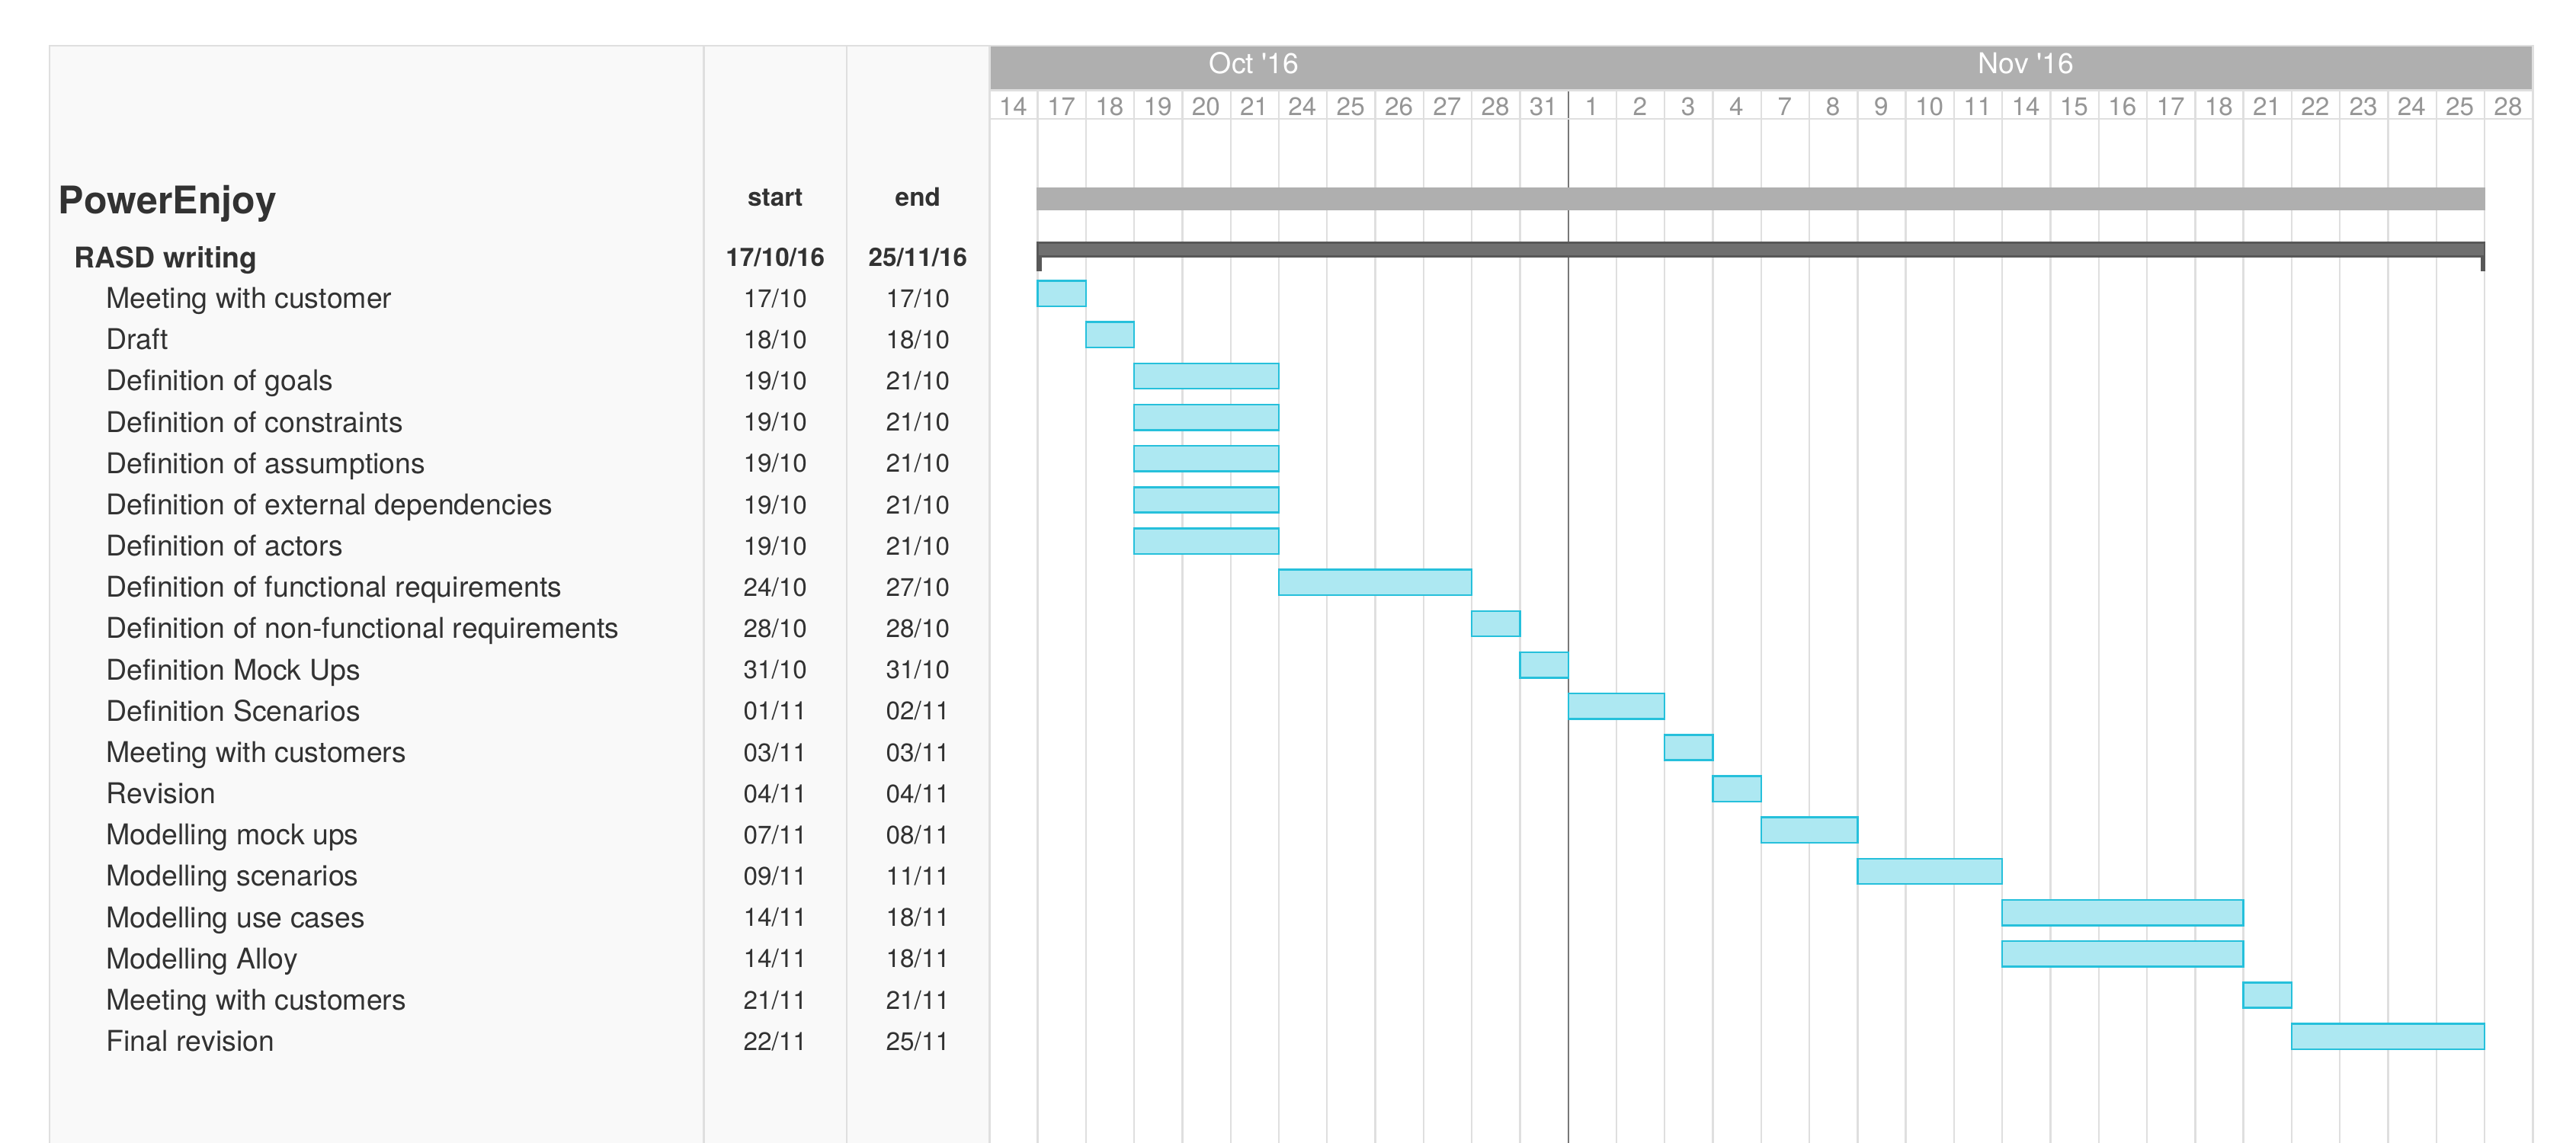
\includegraphics[width=460pt]{RASD-gantt.png}
	}
	\caption{Gantt chart for the RASD writing schedule}
\end{figure}

\subsection{DD writing}

\begin{figure}[H]
	\centering
	\makebox[\textwidth][c]{
		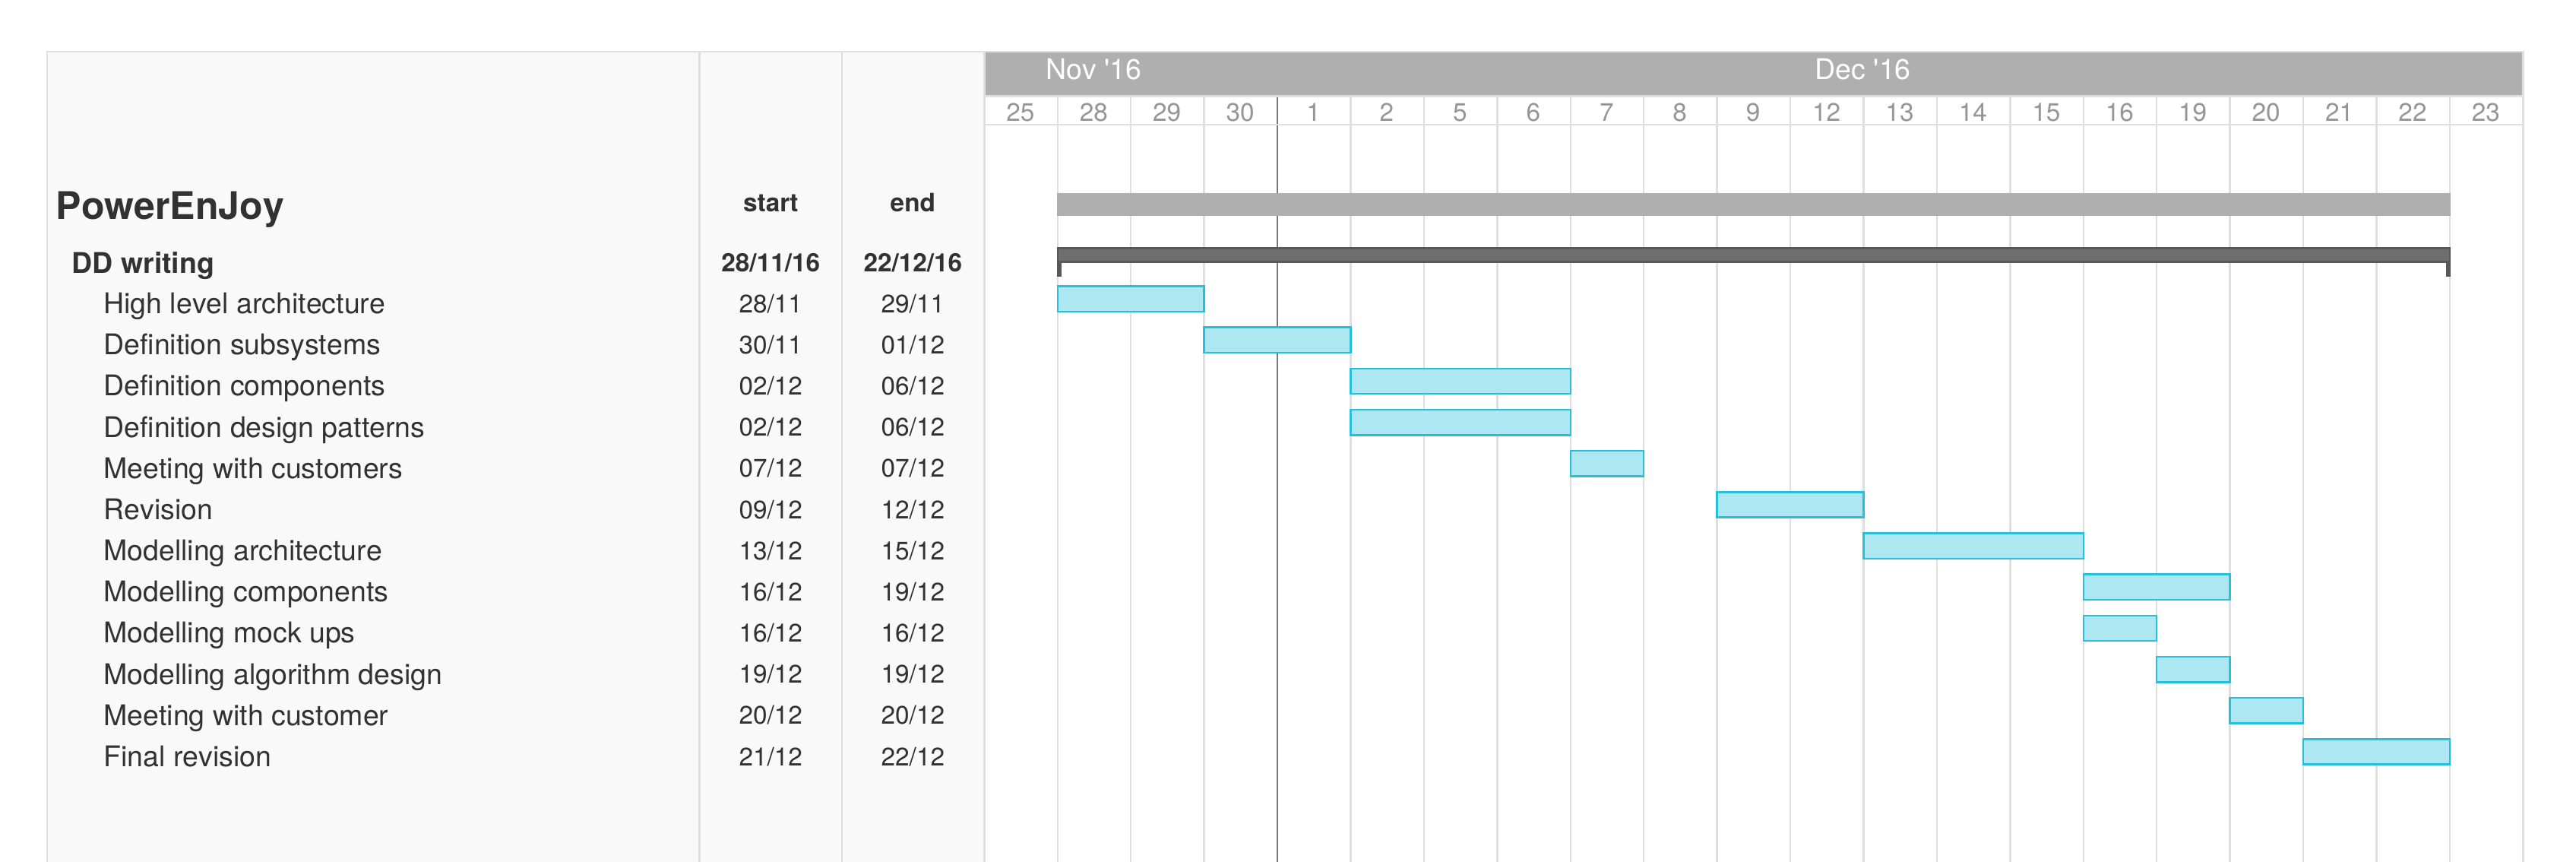
\includegraphics[width=460pt]{DD-gantt.png}
	}
	\caption{Gantt chart for the DD writing schedule}
\end{figure}

\subsection{ITPD writing}

\begin{figure}[H]
	\centering
	\makebox[\textwidth][c]{
		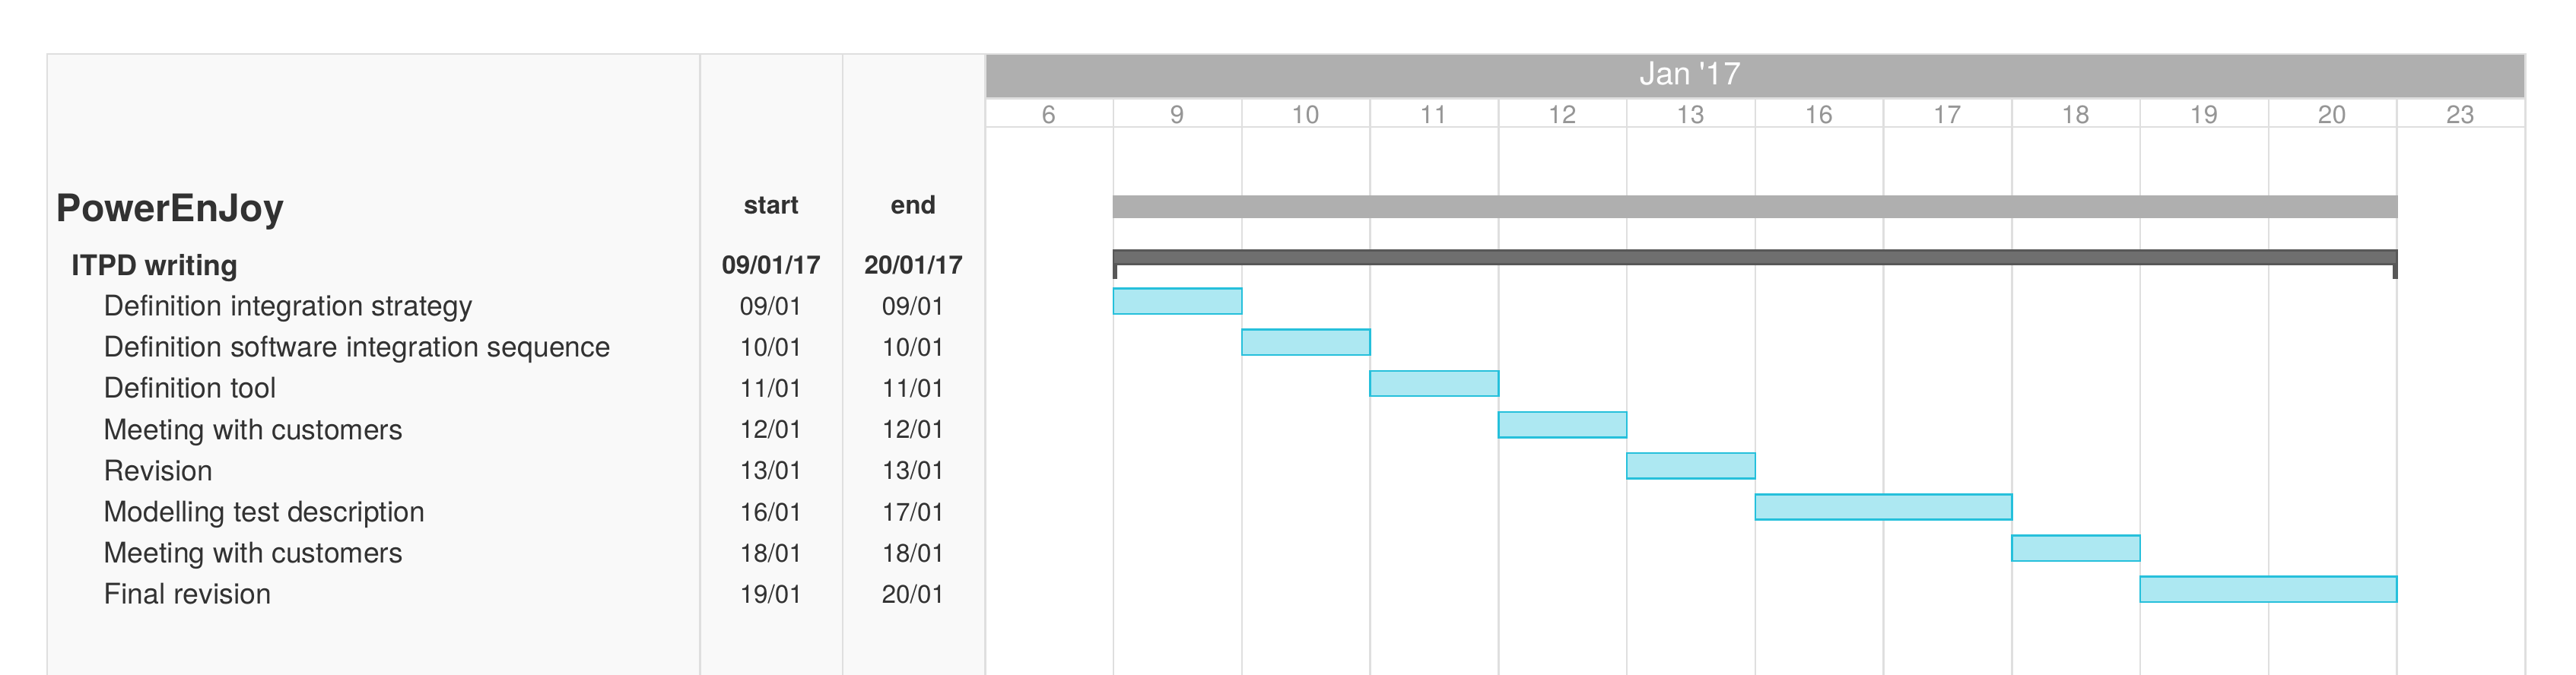
\includegraphics[width=460pt]{ITPD-gantt.png}
	}
	\caption{Gantt chart for the ITPD writing schedule}
\end{figure}

\subsection{Development -- Code Inspection --  Testing}

\begin{figure}[H]
	\centering
	\makebox[\textwidth][c]{
		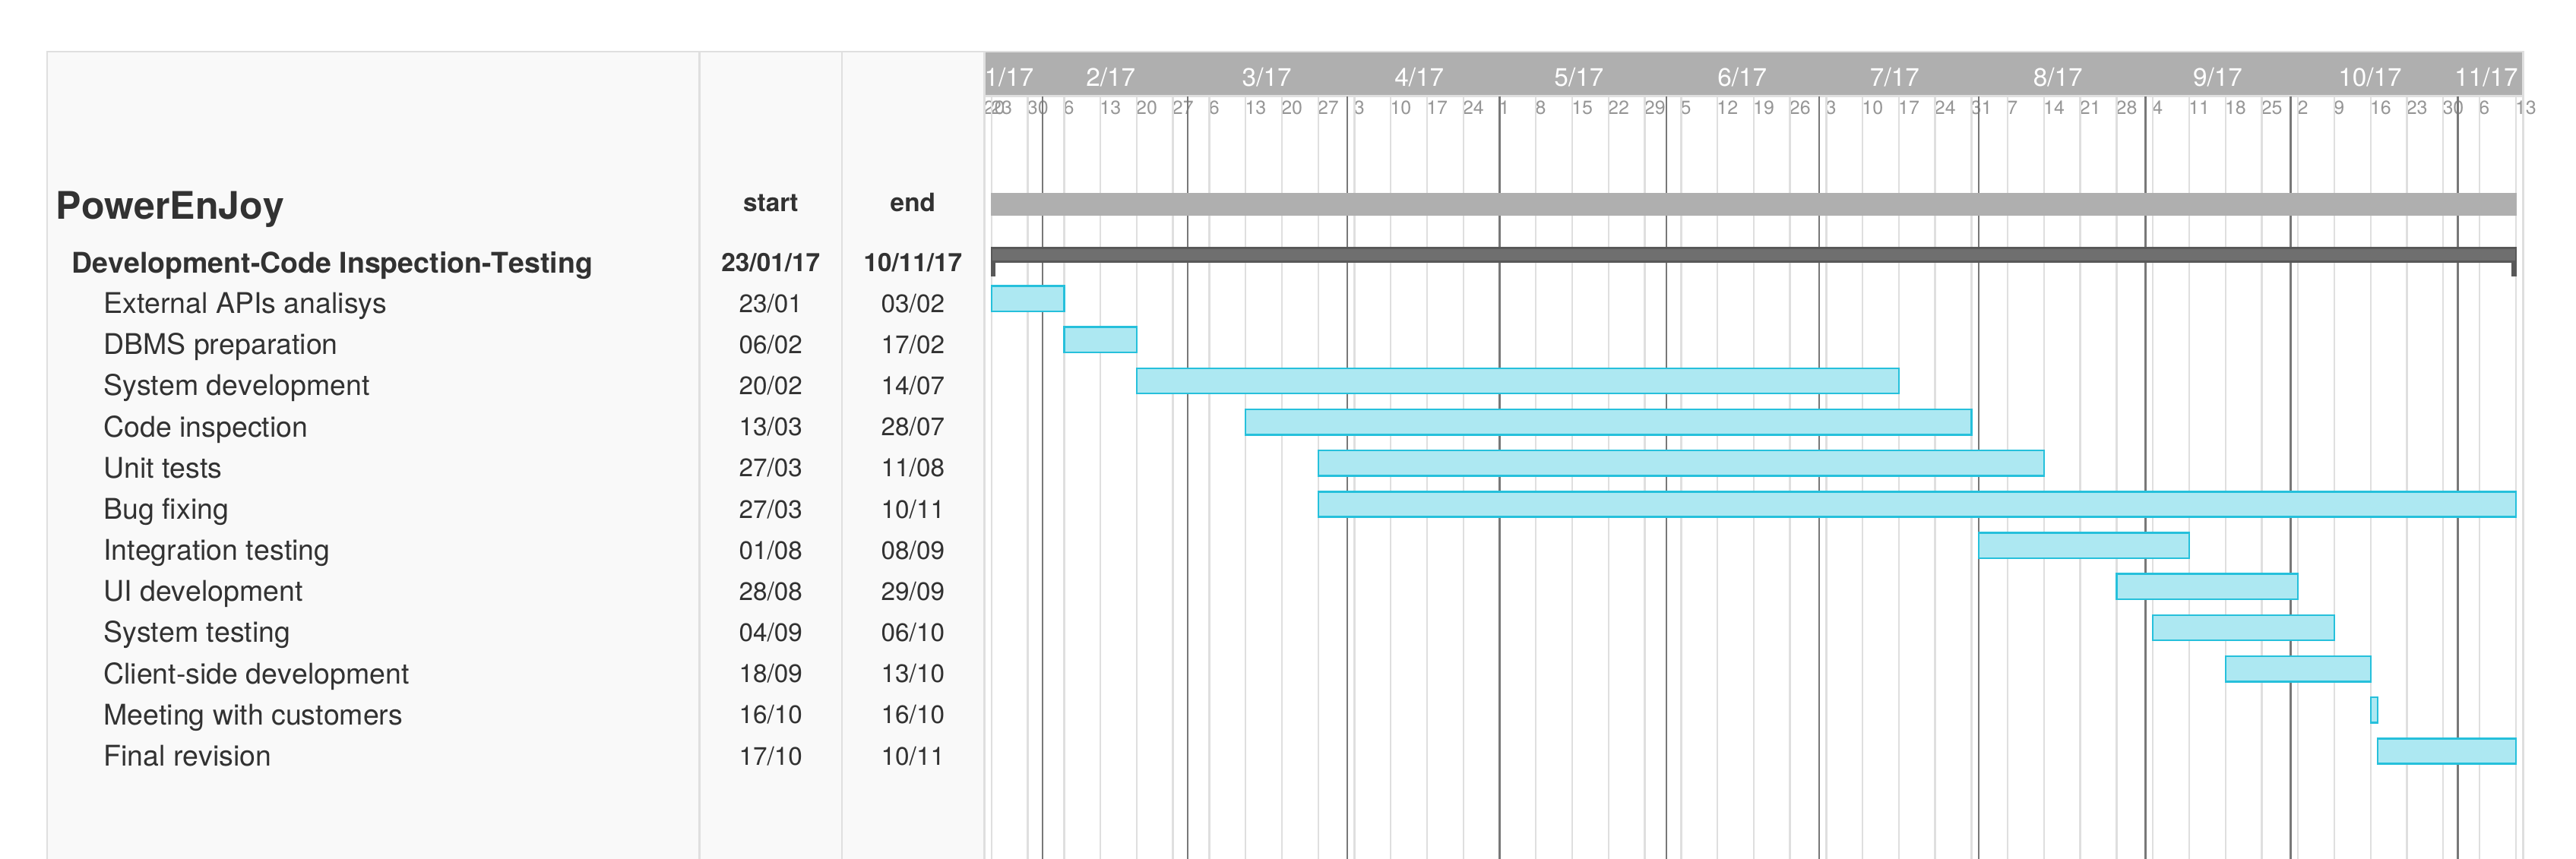
\includegraphics[width=460pt]{development-gantt.png}
	}
	\caption{Gantt chart for the development, code inspection and testing schedule}
\end{figure}

\subsection{Deployment}

\begin{figure}[H]
	\centering
	\makebox[\textwidth][c]{
		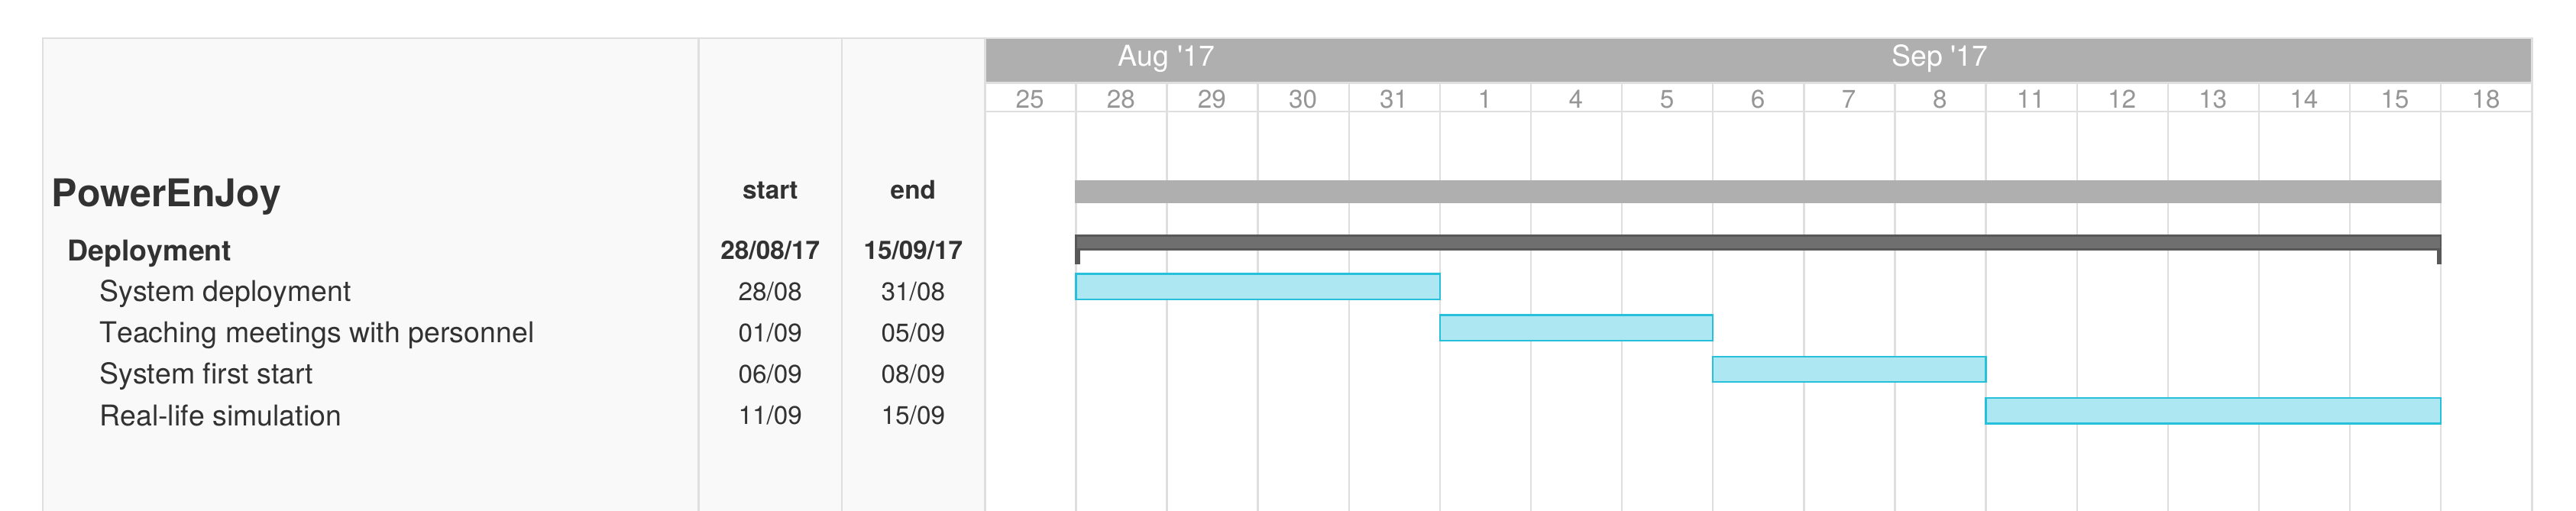
\includegraphics[width=460pt]{deployment-gantt.png}
	}
	\caption{Gantt chart for the deployment schedule}
\end{figure}

\section{Resource allocation}

\paragraph{}

\begin{center}
	\begin{tabular}{|p{3cm}|p{4cm}|}
		\hline
		\multicolumn{2}{|c|}{\textbf{Pietro Ferretti}}\\
		\hline
		RASD Writing & All\\
		\hline
		DD Writing & All\\
		\hline
		ITPD Writing & All\\
		\hline
		Development & External APIs analysis\\
		Code Inspection & DBMS preparation\\
		Testing & System development\\
		& Unit test\\
		& Bug fixing\\
		& Client-side development\\
		& Meeting with customers\\
		& Final revision\\
		\hline
		Deployment & All\\
		\hline		
	\end{tabular}
\end{center}

\begin{center}
	\begin{tabular}{|p{3cm}|p{4cm}|}
		\hline
		\multicolumn{2}{|c|}{\textbf{Nicole Gervasoni}}\\
		\hline
		RASD Writing & All\\
		\hline
		DD Writing & All\\
		\hline
		ITPD Writing & All\\
		\hline
		Development & External APIs analysis\\
		Code Inspection & DBMS preparation\\
		Testing & System development\\
		& Integration testing\\
		& Bug fixing\\
		& UI development\\
		& Meeting with customers\\
		& Final revision\\
		\hline
		Deployment & All\\
		\hline
	\end{tabular}
\end{center}

\begin{center}
	\begin{tabular}{|p{3cm}|p{4cm}|}
		\hline
		\multicolumn{2}{|c|}{\textbf{Danilo Labanca}}\\
		\hline
		RASD Writing & All \\ 
		\hline
		DD Writing & All \\ 
		\hline
		ITPD Writing & All \\ 
		\hline
		Development & External APIs analysis\\ 
		Code Inspection & DBMS preparation\\ 
		Testing & System development\\ 
		& System testing\\
		& Bug fixing\\ 
		& Client-side development\\ 
		& Meeting with customers\\ 
		& Final revision\\
		\hline
		Deployment & \\
		\hline
	\end{tabular}
\end{center}

\newpage
\section{Risk Management}
Risk management is the identification, assessment, and prioritization of risks followed by coordinated and economical application of resources to minimize, monitor, and control the probability and/or impact of unfortunate events.\\
In this section we list PowerEnjoy project's main risks and outline possible strategies to handle the most critical ones.


\begin{center}
	\begin{tabular}{|p{7cm}|p{2cm}|p{2cm}|}
		\hline
		\multicolumn{1}{|c|}{\textbf{Risk}} & \multicolumn{1}{c|}{\textbf{Probability}} & \multicolumn{1}{c|}{\textbf{Impact}} \\
		\hline
		Personnel shortfall (recruitment issues, employee illness or accidents, ...)& moderate & catastrophic\\
		\hline
		Inaccurate Requirements & moderate & critical\\
		\hline
		Unrealistic Schedule & moderate & critical\\
		\hline
		Unrealistic Budget & moderate & critical\\
		\hline
		Stakeholder commitment loss & low & critical\\
		\hline
		New car rental laws & low & catastrophic \\
		\hline
		Inability to obtain proper permits from authorities  & low & catastrophic \\
		\hline
		Inability to obtain a deal with a mobile data provider  & low & critical \\
		\hline		
		Issues with hardware supplier (wrong or defected items, late deliveries, ...) & moderate & critical \\
		%nfrastruttura? 
		%poco successo col pubblico non 
		\hline
		Wrong user interface & moderate & critical\\
		\hline
	\end{tabular}
\end{center}

\paragraph{}

\paragraph{Strategies:}
\begin{itemize}

\item \textit{Personnel shortfall:} reorganize the team so that there is more overlap of work and no single person is fundamental to the project; in case of issues in finding high qualified workers consider buying already developed products and simply adapting them.

\item \textit{Issue with hardware supplies:} use and test hardware components as soon as they are available; replace potentially defective components with bought-in components of known reliability.

\item \textit{Inaccurate requirements:} derive traceability information to assess requirements change impact; divide software functions in several different module so that modify a requirements will not have effect on all the produced code. 

\item \textit{Stakeholder commitment loss:} prepare a briefing document showing how the project is making a very important contribution to the goals of the business.

\item \textit{Unrealistic budget:} have it reconsidered by showing to the stakeholder how the project is making a very important contribution to the goals of the business; buy already developed products and assembly them. 

\item \textit{Unrealistic schedule:} early in the development, divide bigger activities in smaller ones and hired new people to work on few specific functions then combine them when ready, while later consider buying already developed products and adapting them.
\end{itemize}


\appendix
\newpage

\section{Hours of work}

\begin{itemize}
	\item{Pietro Ferretti: 15 hours of work}
	\item{Nicole Gervasoni: 10 hours of work}
	\item{Danilo Labanca: 20 hours of work}
\end{itemize}

\section{Changelog}

\begin{itemize}
	\item PP v1.0, published on January 22, 2017
\end{itemize}

\end{document}
